\section{System design}
In this chapter, the design of the system is explained.
The focus of section 3.1 will be an overview of the first approach implemented, the ring topology. Here, a detailed analysis this architecture and its tradeoffs is presented. Similarly, in section 3.2 there is an analysis of the second approach implemented with full connectivity. Lastly, in section 3.3 we discuss the additional features implemented in the system. \\\\
All the components of the system have been written using Java 8, to invoke the remote methods they make use of the Java RMI library which provides a high level of abstraction making the development easier. Instead of implementing a message passing system for the coordination among all the components we made use of the ParSeq library [1] which makes asynchronous communication easier. 

\subsection{Ring topology}

The proposed architecture, depicted in figure 1, consists on a logical ring of GSs and evenly divided groups of RMs.
Each group of RMs is primarily connected to one GS (blue lines) and the next GS in the ring as backup (red lines). Apart from that, every GS is connected to the next and previous GS of the logical ring (black lines). Being connected means to send periodically heartbeats to check if the components are online. 
\\ 
\begin{figure}[H]
\centering
	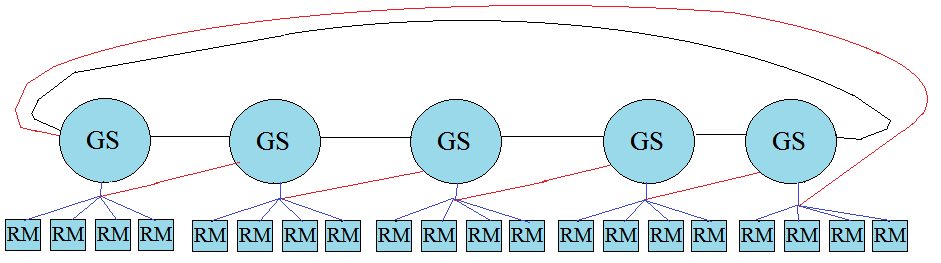
\includegraphics[scale=0.62]{ring.png}
	\caption{Ring topology}
\end{figure}

\subsubsection{Bootstrap}
As in most of distributed computing systems [ref], this topology has the bootstrap problem. How to initiate the system? Since the topology is fixed, the components need to know previously with who they are going to be connected with which causes new synchronization issues.

\subsubsection{Replication}
When a job request arrives to a cluster controlled by a RM this will check whether it can accept the job or not. If there are resources available, the RM will send a monitoring request to its main GS, once it gets confirmation, it will send a backup monitoring request to its backup GS. After receiving confirmation from both grid schedulers, it will begin the execution of the job in one of its nodes. This replication strategy guarantees that if a RM suspends its activity, the jobs can be rescheduled in another cluster and that in case of failure of one GS or GS/RM at the same time, the remaining GS will be able to reallocate the workload of the failed cluster in another one.

\subsubsection{Fault recovery}
Failures of RM are discovered by the main GS, when this happens the GS will reallocate the jobs in another cluster and inform the backup GS to stop monitoring the previous RM. After that, the new RM will request to its main and backup GS monitoring for the workload received just as if they were normal job requests. Once monitoring is received, it will start the execution.
On the other hand, when the backup GS detects the failure of the main GS, it will self promote to become the main GS of the cluster under the control of the failed GS. Additionally, the RM will connect to the previous GS on the ring next to the failed one as backup GS.
\\\\
This strategy of fault recovery may seem robust, however, it is likely to trigger a failure of the whole system due to the domino effect. The reason behind it is that all the workload monitored by the failed GS is supported by backup. If the latter has already a big amount of jobs under its supervision, it will probably fail as well triggering a domino failure. This scenario is also possible in the case of a RM failure. The GS monitoring the new selected cluster will assume all the incoming workload. Moreover, given that when a node crashes all its connections are re-established it is hard to implement the "coming back to life" mechanism.
